\documentclass[12pt]{article}
%\documentclass{article}

\usepackage{times}
\usepackage[final]{graphicx}
\usepackage{hyperref}

\setlength{\topmargin}{-0.5in}
\setlength{\oddsidemargin}{0in}
\setlength{\evensidemargin}{0in}
\setlength{\textwidth}{6.5in}
\setlength{\textheight}{9.0in}

\begin{document}

\centerline{\bf \Large CS295/CS395/CSYS395: \href{CS295_395_Syllabus.pdf}{\underline{Evolutionary Robotics}}}

\vspace{0.5cm}

\centerline{\bf \large Programming Assignment 1 of 10}

\vspace{0.5cm}

\centerline{\large Assigned: Friday, September 2, 2011}

\vspace{0.5cm}

\centerline{\large Due: Friday, September 9, 2011 by midnight}

\vspace{0.5cm}

\noindent \textbf{Description:} The field of evolutionary robotics is so called because in a typical experiment, an \underline{evolutionary algorithm} is used to automatically optimize robots so that they perform a desired task. There are many kinds of evolutionary algorithms, but they all share one thing in common: they are a simplified model of how biological evolution works. In short, in any evolutionary algorithm (1) the fitness of each entity in an intially random population is measured; (2) those entities with lower fitness are discarded; (3) modified copies of those that remain are made; (4) the fitness of each new entity is measured; and (5) this cycle repeats until a highly fit entity is discovered. \\

In this assignment you will be creating the simplest evolutionary algorithm, a serial hill climber. The algorithm is known as a hill climber because one can imagine the space of all entities that are to be searched as lying on a surface, such that similar entities are near one another. The height of the surface at any one point indicates the quality, or fitness of the entity at that location. This is known as a
\href{http://en.wikipedia.org/wiki/Fitness_landscape}
{\underline{fitness landscape}}. A hill climber gradually moves between nearby entities and always moves `upward': it moves from an entity with lower fitness to a nearby entity with higher fitness. \\

In this assignment, rather than evolving robots, you will simply evolve vectors of the form $v = {e_1, \ldots e_n}$, where the $i$th element in the vector may take on a real number in $[0,1]$. The fitness of a vector $v$, denoted $f(n)$ we will define as the mean value of all of its elements:
\begin{eqnarray}
f(v) = \frac{\sum_{i=1}^{n}e_i}{n}
\end{eqnarray}
Thus, the hill climber will search for vectors in which all of the elements have values near one. In assignment 3, you will re-use the hill climber you develop here to evolve neural networks; in assignment 10, you will use it to evolve robots. \\

\noindent \textbf{Tasks:}

You will be creating the hill climber in Python. If you are not familiar with Python, this assignment will serve as a good introduction to the language.

\begin{enumerate}

\item Download, install and run \href{http://www.python.org/}{\underline{Python}}, an open source language available for most computing platforms. \textbf{You are free to do all of the programming assignments in a Mac, Windows or Linux environment.} In order to make sure you installed Python correctly, work through the first 10 minutes of any online Python tutorial.

\item In order to use vectors and matrices in Python you will also need to download and install \href{http://numpy.scipy.org/}{\underline{NumPy and SciPy}}. In order to make sure you installed both of these applications correctly, work through the first 10 minutes of this \href{http://www.scipy.org/Tentative_NumPy_Tutorial}{\underline{tutorial}}.

\item Rather than submitting code to be graded, in this course you will submit screenshots of graphics that visually demonstrate you have successfully completed the assignment. The three screenshots you will create for this assignment look like those shown in Fig. \ref{Fig}. To create graphics in Python, download and install matplotlib
    (\href{http://matplotlib.sourceforge.net/}
    {\underline{website}} here;
    \href{http://sourceforge.net/projects/matplotlib/files/matplotlib/matplotlib-1.0/}
    {\underline{download}} here),
    a Matlab-similar set of graphing libraries. In order to make sure you installed Matplotlib correctly, copy and paste the code associated with any of the graphs from the site's gallery.

\item The first step in the serial hill climber is to create a random vector. To do this, create a Python function \textbf{\texttt{v = MatrixCreate(1,50)}}. This function should return a vector with 50 elements, all set to zero. The vector is actually a $1 \times 50$ matrix. \textbf{\texttt{print v}} will show you whether the vector was created successfully or not.

\item Create a function \textbf{\texttt{v = MatrixRandomize(v)}} that will put random values drawn from $[0,1]$ into each element of v. You'll need to use \textbf{\texttt{random()}}, which returns a random floating-point value in $[0,1]$.

\item The hill climber must now compute the fitness of the random vector. Create a function \texttt{\textbf{f = Fitness(v)}} that returns the mean value of all of the elements in $v$.

\item The hill climber must now create a modified copy of $v$. Create a function \texttt{\textbf{c = Matrix Perturb(p,0.05)}} which makes a copy of the parent vector $p$, and then considers each element in the new vector $c$. With probability 0.05, the element's value is replaced with a new random value drawn from $[0,1]$; otherwise, the element's value is left as is. You can cause an event to happen with a given probability using an if statement: \textbf{\texttt{if ( random()<0.05 ):}}.

\item You can now use all of these functions to create a serial hill climber: \\
\textbf{\texttt{parent = MatrixCreate(1,50)}}\\
\textbf{\texttt{parent = MatrixRandomize(parent)}}\\
\textbf{\texttt{parentFitness = FitnessParent(parent)}}\\
\textbf{\texttt{for currentGeneration in range(0,5000):}}\\
\indent \textbf{\texttt{\hspace{1cm}print currentGeneration, parentFitness}}\\
\indent \textbf{\texttt{\hspace{1cm}child = MatrixPerturb(parent,0.05)}}\\
\indent \textbf{\texttt{\hspace{1cm}childFitness = Fitness(child)}}\\
\indent \textbf{\texttt{\hspace{1cm}if ( childFitness > parentFitness ):}}\\
\indent \textbf{\texttt{\hspace{2cm}parent = child}}\\
\indent \textbf{\texttt{\hspace{2cm}parentFitness = childFitness}}\\

\item You should see that as the fitness of parent is printed, the fitness value goes up as the generations pass.

\end{enumerate}

\begin{figure}[!t]
\centerline{a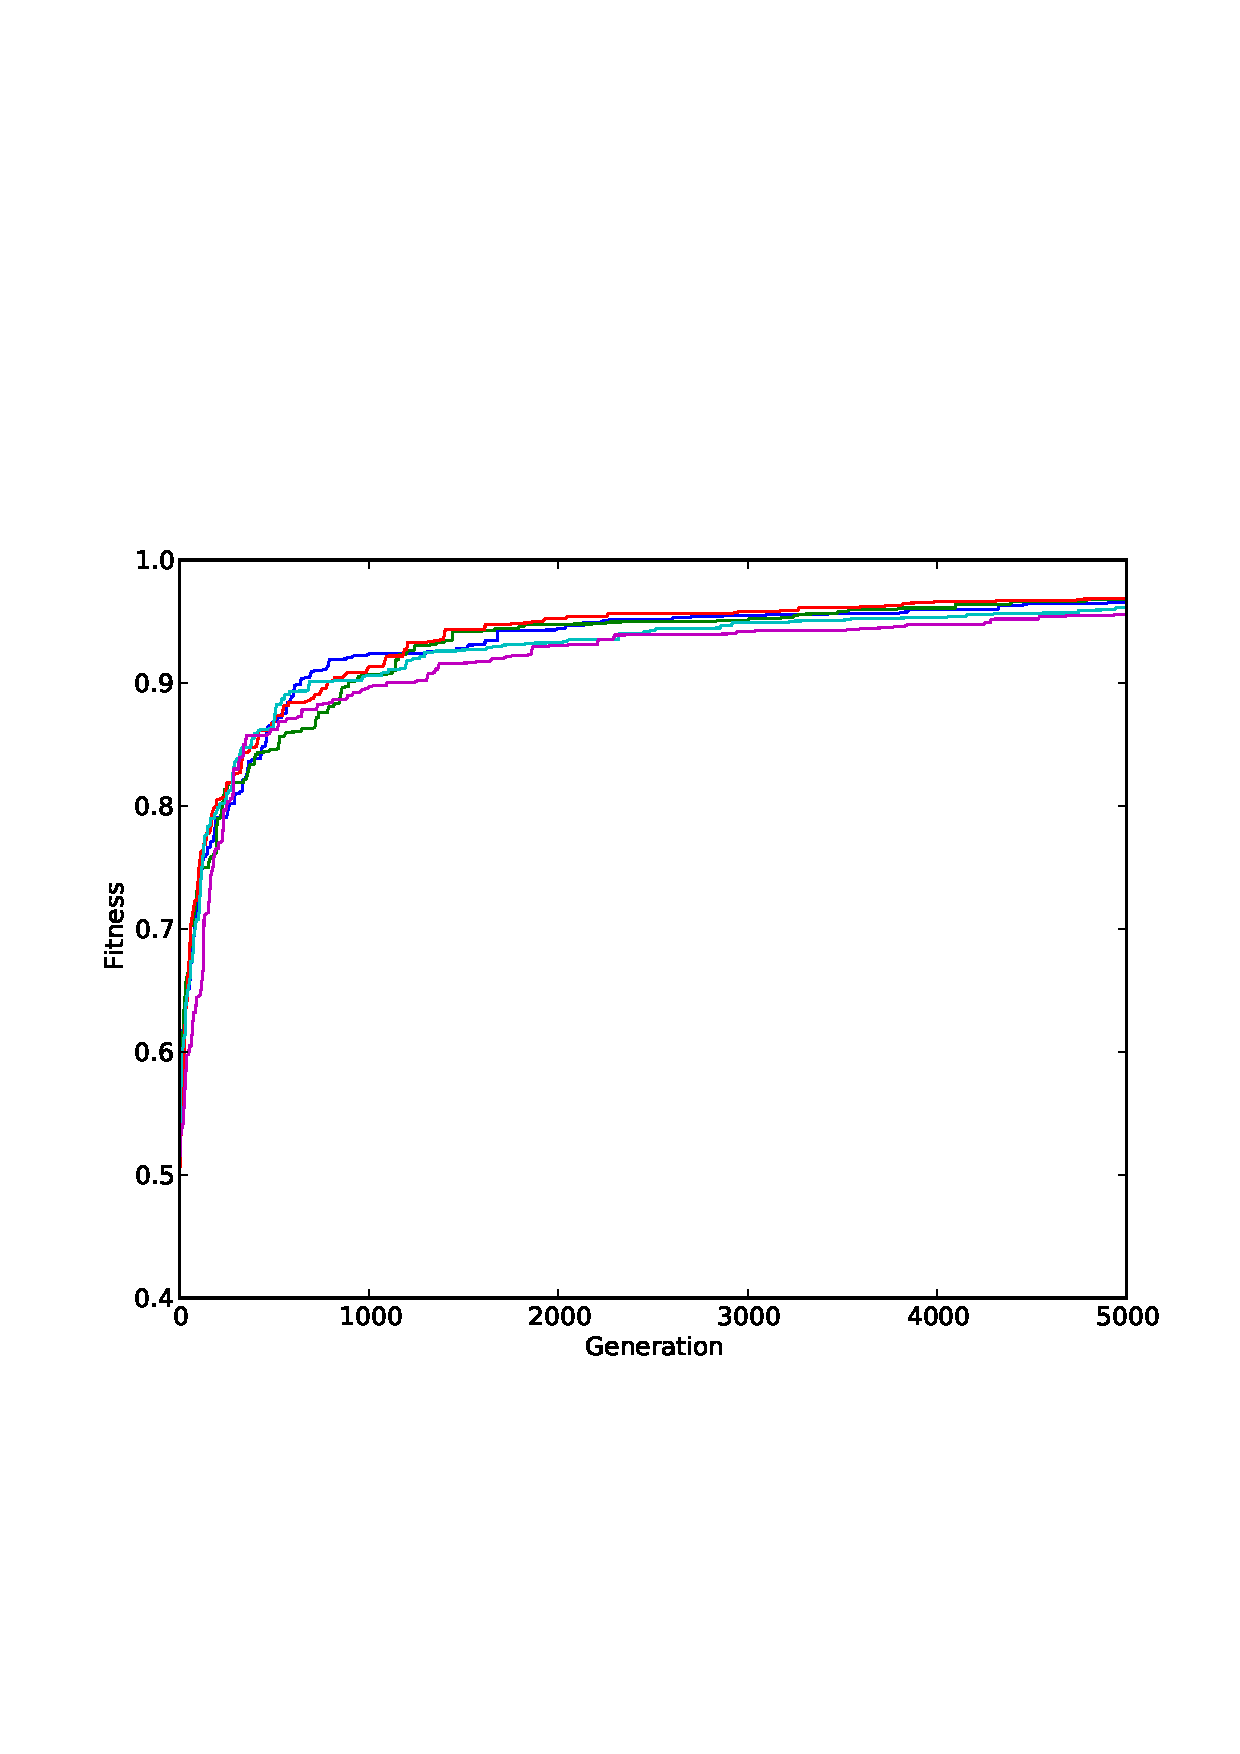
\includegraphics[width=0.75\textwidth]{Fits.pdf}}
\centerline{b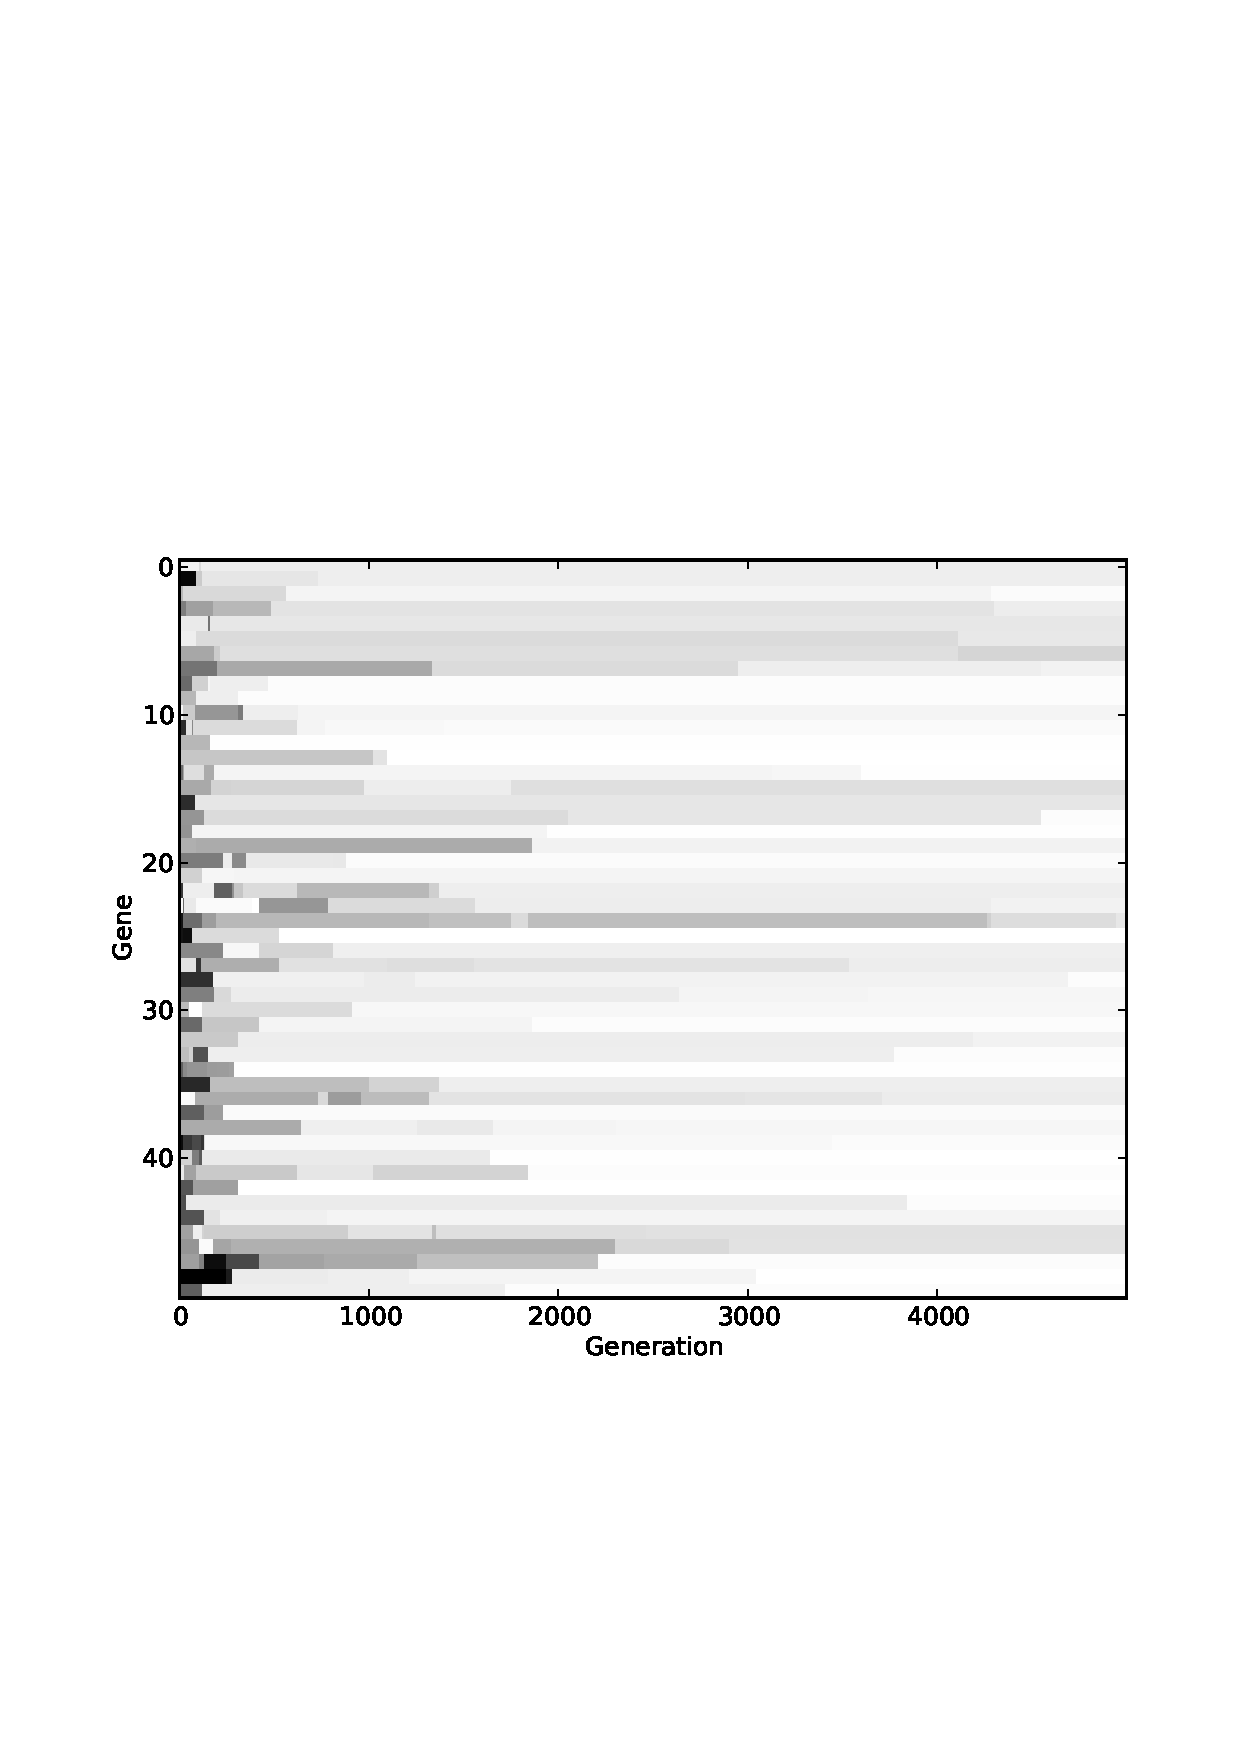
\includegraphics[width=0.75\textwidth]{Genes.pdf}}
\caption{Results from running five serial hill climbers.
a: The fitness curves for the five runs.
b: The values of the 50 genes in the vector: lighter values indicate higher values.}
\label{Fig}
\end{figure}

\noindent \textbf{Deliverables:}

\begin{enumerate}

\item The first graph you will create will visually show how the fitness of the best vector climbs as the generations pass. In your existing code, create a new vector \textbf{\texttt{fits = MatrixCreate(1,5000)}} that stores the fitness value of the parent at each generation. Print \textbf{\texttt{fits}} after your code has run to make sure the fitness values have been stored.

\item Create a function \textbf{\texttt{PlotVectorAsLine(v)}} that plots the vector as a line (use \textbf{\texttt{plot()}} from matplotlib). The graph should show one line with a curve similar to those of the lines in Fig. \ref{Fig}a. Save this figure, and paste it into either a Word document or a \href{http://www.latex-project.org/}{\underline{Latex}} document.

\item Wrap the Python code from step 8 above in a loop that runs the hill climber five times, each time starting with a different random vector. At the end of each pass through the loop, add another line to your graph, so that you have a picture similar to that in Fig. \ref{Fig}a.

\item Create a matrix \textbf{\texttt{Genes}} with 5000 columns and 50 rows. After each generation $j$ of the hill climber, copy each element of the parent vector into the $j$th column of \textbf{\texttt{Genes}}. After the hill climber has run, \textbf{\texttt{print Genes}} to ensure the elements were stored correctly.

\item The matplotlib function \textbf{\texttt{imshow(M)}} will print a matrix $M$ as an image, where each pixel $p_{ij}$ corresponds to element $e_{ij}$ in $M$. Calling \textbf{\texttt{imshow(Genes}}, \textbf{\texttt{cmap=cm.gray}}, \textbf{\texttt{aspect='auto'}}, \textbf{\texttt{interpolation='nearest')}} after the hill climber has terminated will produce a figure similar to that of Fig. \ref{Fig}b. \textbf{\texttt{cmap=cm.gray}} will ensure that the image is shown in grayscale: elements with values near 1 will be plotted as near-white pixels; elements near zero will be plotted as near-black pixels. \textbf{\texttt{aspect='auto'}} will expand the otherwise very long, flat image to fill the figure window. \textbf{\texttt{interpolation='nearest'}} will stop any blurring between the pixels.

\item Copy and paste the resulting figure into your document with the other two figures. Now, convert your document to pdf using a pdf conversion application such as \href{http://www.primopdf.com/index.aspx}{PrimoPDF}. Email the pdf to the TA.

\end{enumerate}

\noindent \textbf{Notes:}

\begin{enumerate}
\item For those of you working on a Mac, the order in which you install the Python packages matters. From the command line on a Mac:\\
    \texttt{python} \\
    \texttt{>>> import scipy} \\
    \texttt{>>> import numpy} \\
    \texttt{>>> import matplotlib} \\
    Do not \texttt{install matplotlib.pyplot}; you can call the matplotlib routines after installing these three packages
\end{enumerate}

\end{document} 
